\documentclass[12pt,UTF8]{ctexbook}

\input{../common/page}

\xeCJKsetup{AutoFallBack=true}
\setCJKfamilyfont{hei}{SimHei}
\setCJKfamilyfont{kai}{KaiTi}

\usepackage{titletoc}
\titlecontents{chapter}[0pt]{\vspace{3mm}\bf\addvspace{2pt}\filright}{\contentspush{\thecontentslabel\space}}{}{\titlerule*[8pt]{.}\contentspage}

\usepackage[colorlinks,linkcolor=blue,citecolor=blue,urlcolor=blue]{hyperref}

\ctexset{
	part/name= {第,卷},
	part/number={\chinese{part}},
	chapter/name={第,章},
	chapter/number={\arabic{chapter}}
}

\usepackage{graphicx}
\graphicspath{{AV女优_images/}}

\newenvironment{shuming}{\hfill\zihao{4}}

\usepackage[perpage]{footmisc}

\newenvironment{yuanwen}{\bfseries\zihao{4}}

\setlength{\parskip}{0.8em plus 0.2em minus 0.1em}

\usepackage{enumitem}

\title{\heiti\zihao{0} AV女优的工作现场}
\author{溜池五郎 著 王榆琮 译}
\date{\today}

\begin{document}

\maketitle
\tableofcontents

\frontmatter
\chapter{前言}

我20岁时曾担任过电视剧和电影的导演助理，但并不是制作公司、电视台的正职人员，只是区区一名约聘雇员。从大学毕业至今，也从未像个上班族般正式工作过，总是漂泊不定地四处讨生活，只要工作有趣，我就会投身其中，当然，我个人认为这种状态，好坏参半。

~\\

\section{比一般工作更有趣}

20年前，透过某个独立电影的制作工作，我经由一位前辈级的影像作家介绍，结识了成人影视圈的征才人员，也因此敲开了A片界的大门。我还记得当时自己会想进入这个圈子，就是觉得这一行比当导演助理还要有趣得多。

1994年，水沼纱英（化名/当时20岁）的作品成为我正式执导的处女作。在那部作品中，不只使用专门拍摄电视剧的场景，而且在演出、运镜手法上也维持拍摄电视剧的规格。这后来在业界成了所谓的「戏剧型」A片，也因此在圈内博得好评。

至于溜池五郎这个名号当然是艺名，而帮我取这个名字的人正是大名鼎鼎的超级AV男优——加藤鹰先生。

之所以会取这个名字，只是因为相关制作公司的办公室在东京都港区溜池。当初我一听到这个名字就觉得「未免也太奇怪了……」，但毕竟出主意的人是这一行的前辈，说什么都不容违抗。虽然心不甘情不愿地接受这个名字，但当时的我怎么也没想到，这个名字居然能陪我走过20年。

我在事业上的转捩点则是在1999年。那一年高桥雅也先生设立全新的A片公司——Soft On Demand。当时，A片的流通还停留在批发商贩售影带至出租店再出租给消费者的形式，Soft On Demand的「影带销售」模式，也就是制作直接在店面中贩售给消费者的A片，为当时的业界带来一股新气象。

\section{心血操纵在导演手上}

「影带销售」的定价通常约莫在4000至6000日圆上下，即使与现代的经济水准相比，也不是便宜的价格，但却紧紧抓住早已无法从制式化A片中感受到魅力的消费者心意。

不但要有前瞻性的企划，同时也得打破过去A片的窠臼。而之所以能在这些满腔热情的作品中注入如此坚强的阵容，其实是因为高桥先生曾对我说过：

「A片全都操纵在导演手上。」

当年我提出的企划在新进导演中，也算是散发独特个人色彩的类型，因为我只起用熟女来当作拍片主角。在A片业界，只要是27岁以上的女优，都会被当成没有任何商品价值的「大婶级」演员，而我的作法可以说是引起一股划时代风潮。

任谁都没料到，我的熟女A片居然能热卖，而美丽的熟女，也就是「美熟女」正是其中致胜关键。平均一部就能有超过一万片的销售量，这在当时与现在都算是销售数字极为令人满意的畅销作品。

\section{拥有旺盛生命力的女性}

从初次拍片以来，我所导演过的A片至今已经超过1000部，确切的数据连我自己也没办法清楚掌握。在这期间我看过许多AV女优，其中一位日后甚至还成了我的妻子。

虽然我说成人影片是我一生的良师益友，但这个社会还是只看到我投身于将性爱当成商品的世界，只将我定位成特立独行的异端分子。也许和一名前AV女优的女性共结连理，就普世价值而言，正是属于相对不正常的情况，但我反而认为正是这种价值观，才会让大家对AV女优产生各种误解。

我能理解为何靠脱衣赚钱的女人会被他人投以异样眼光，但是从我在摄影现场接触到的女优们中发现，她们的表现并不如同一般人的印象那样。例如我的妻子，过去不仅经济独立，面对工作时的敬业态度更堪称职业级水准。当AV女优离开萤幕焦点后，也一样会有家人、情人、丈夫以及自己的孩子相伴，其中更不乏是拥有旺盛生命力的坚强女性，也能够同时兼顾其他一般工作。

\section{A片也是一种「创作」}

本书绝对不是专门爆料隐私的狗仔情报，而是一本公开女优、业界人士真实样貌的书籍。

虽然这个社会看待AV女优仍然停留在私生活糜烂，只要有钱就能和男人上床的刻板印象上，但在这边我还是要再度强调，事实并非如此。

大多数人的确都能在网路上的影片、DVD里，轻易看到女优们脱光衣服、娇喘不已——虽然她们相当习惯在众人面前轻解罗衫——但再怎么说，这也只不过是一种「工作态度的展现」而已。

我这么一说，其他AV界人士应该会觉得这种话会破坏粉丝对AV女优的憧憬，只会让粉丝觉得：「怎么会这么现实，亏我还很欣赏某某女优那种好色的模样。」然而，我却不这么认为。因为粉丝若是真心支持这个业界的消费者，也许早就已经充分理解A片是一种「创作」，我反到认为消费者看待创作一直都非常耳清目明。

\section{改变社会对A片的看法}

说起来，现在的A片确实越来越难卖。其中理由所在多有，例如：电脑的普及、年轻男性对女性的兴趣降低，开始出现一股草食男趋势等等（其实，DVD主要客群以中老年人为多）。另外，我们这些负责创作的业界人士，一直死板看待粉丝对A片的憧憬也是原因之一。

从另一个角度看来表示我所处的AV业界，仍打从心里认为消费者无论如何都能无条件相信，A片业界所创造出来的幻想，但这在本质上其实就是一种瞧不起消费者的心态。

我认为现在正是A片业界开诚布公的时期，透过让大家了解AV女优和一般人无异，也许多少能改变这个社会对A片的看法。

所以在我写这本书时，就打算用比较具体的方式写出我在现场亲眼看见、亲身经历的故事。不过，本书仍然只是我个人在业界所经历到的各种人事物，确实不足以代表整个A片界，这点还请各位多多包涵。

\mainmatter

\chapter{内容简介}

熟女系AV大导演溜池五郎以20多年的AV执导经历，绝对有资格告诉你，你所不知道的情色影片现场的真实样貌。

巨乳靠天生，美臀靠态度。在淫声浪语的背后，是无人能及的专业素养；大众有色的眼光下，面对的是不亚于你我的职场激烈竞争。

【你不知道的是】只要躺着干就好？AV女优是全世界职场环境最严苛的职业之一，一年有八成女优惨遭淘汰！

【你不知道的是】天生丽质才出道？这里有比艺能界、模特界更严苛的美体标准！

【你不知道的是】口袋空空真难熬？她们大多数都是现役护士、老师、OL甚至企业老板！

【你不知道的是】学历不高刚刚好？近来的AV女优不乏高学历者，甚至有许多人只是想寻求刺激、留下一个青春回忆！

【你不知道的是】年轻貌美是王道？熟女、超熟女等姊姊们也各有死忠粉丝，拥有不可思议的熟龄魅力！

【你不知道的是】恋情谢绝窝边草？AV女优当然会谈恋爱，而且偶尔来场「办公室恋情」也不意外！

\chapter{第1章 AV女优}

\begin{figure}[htbp]
	\centering
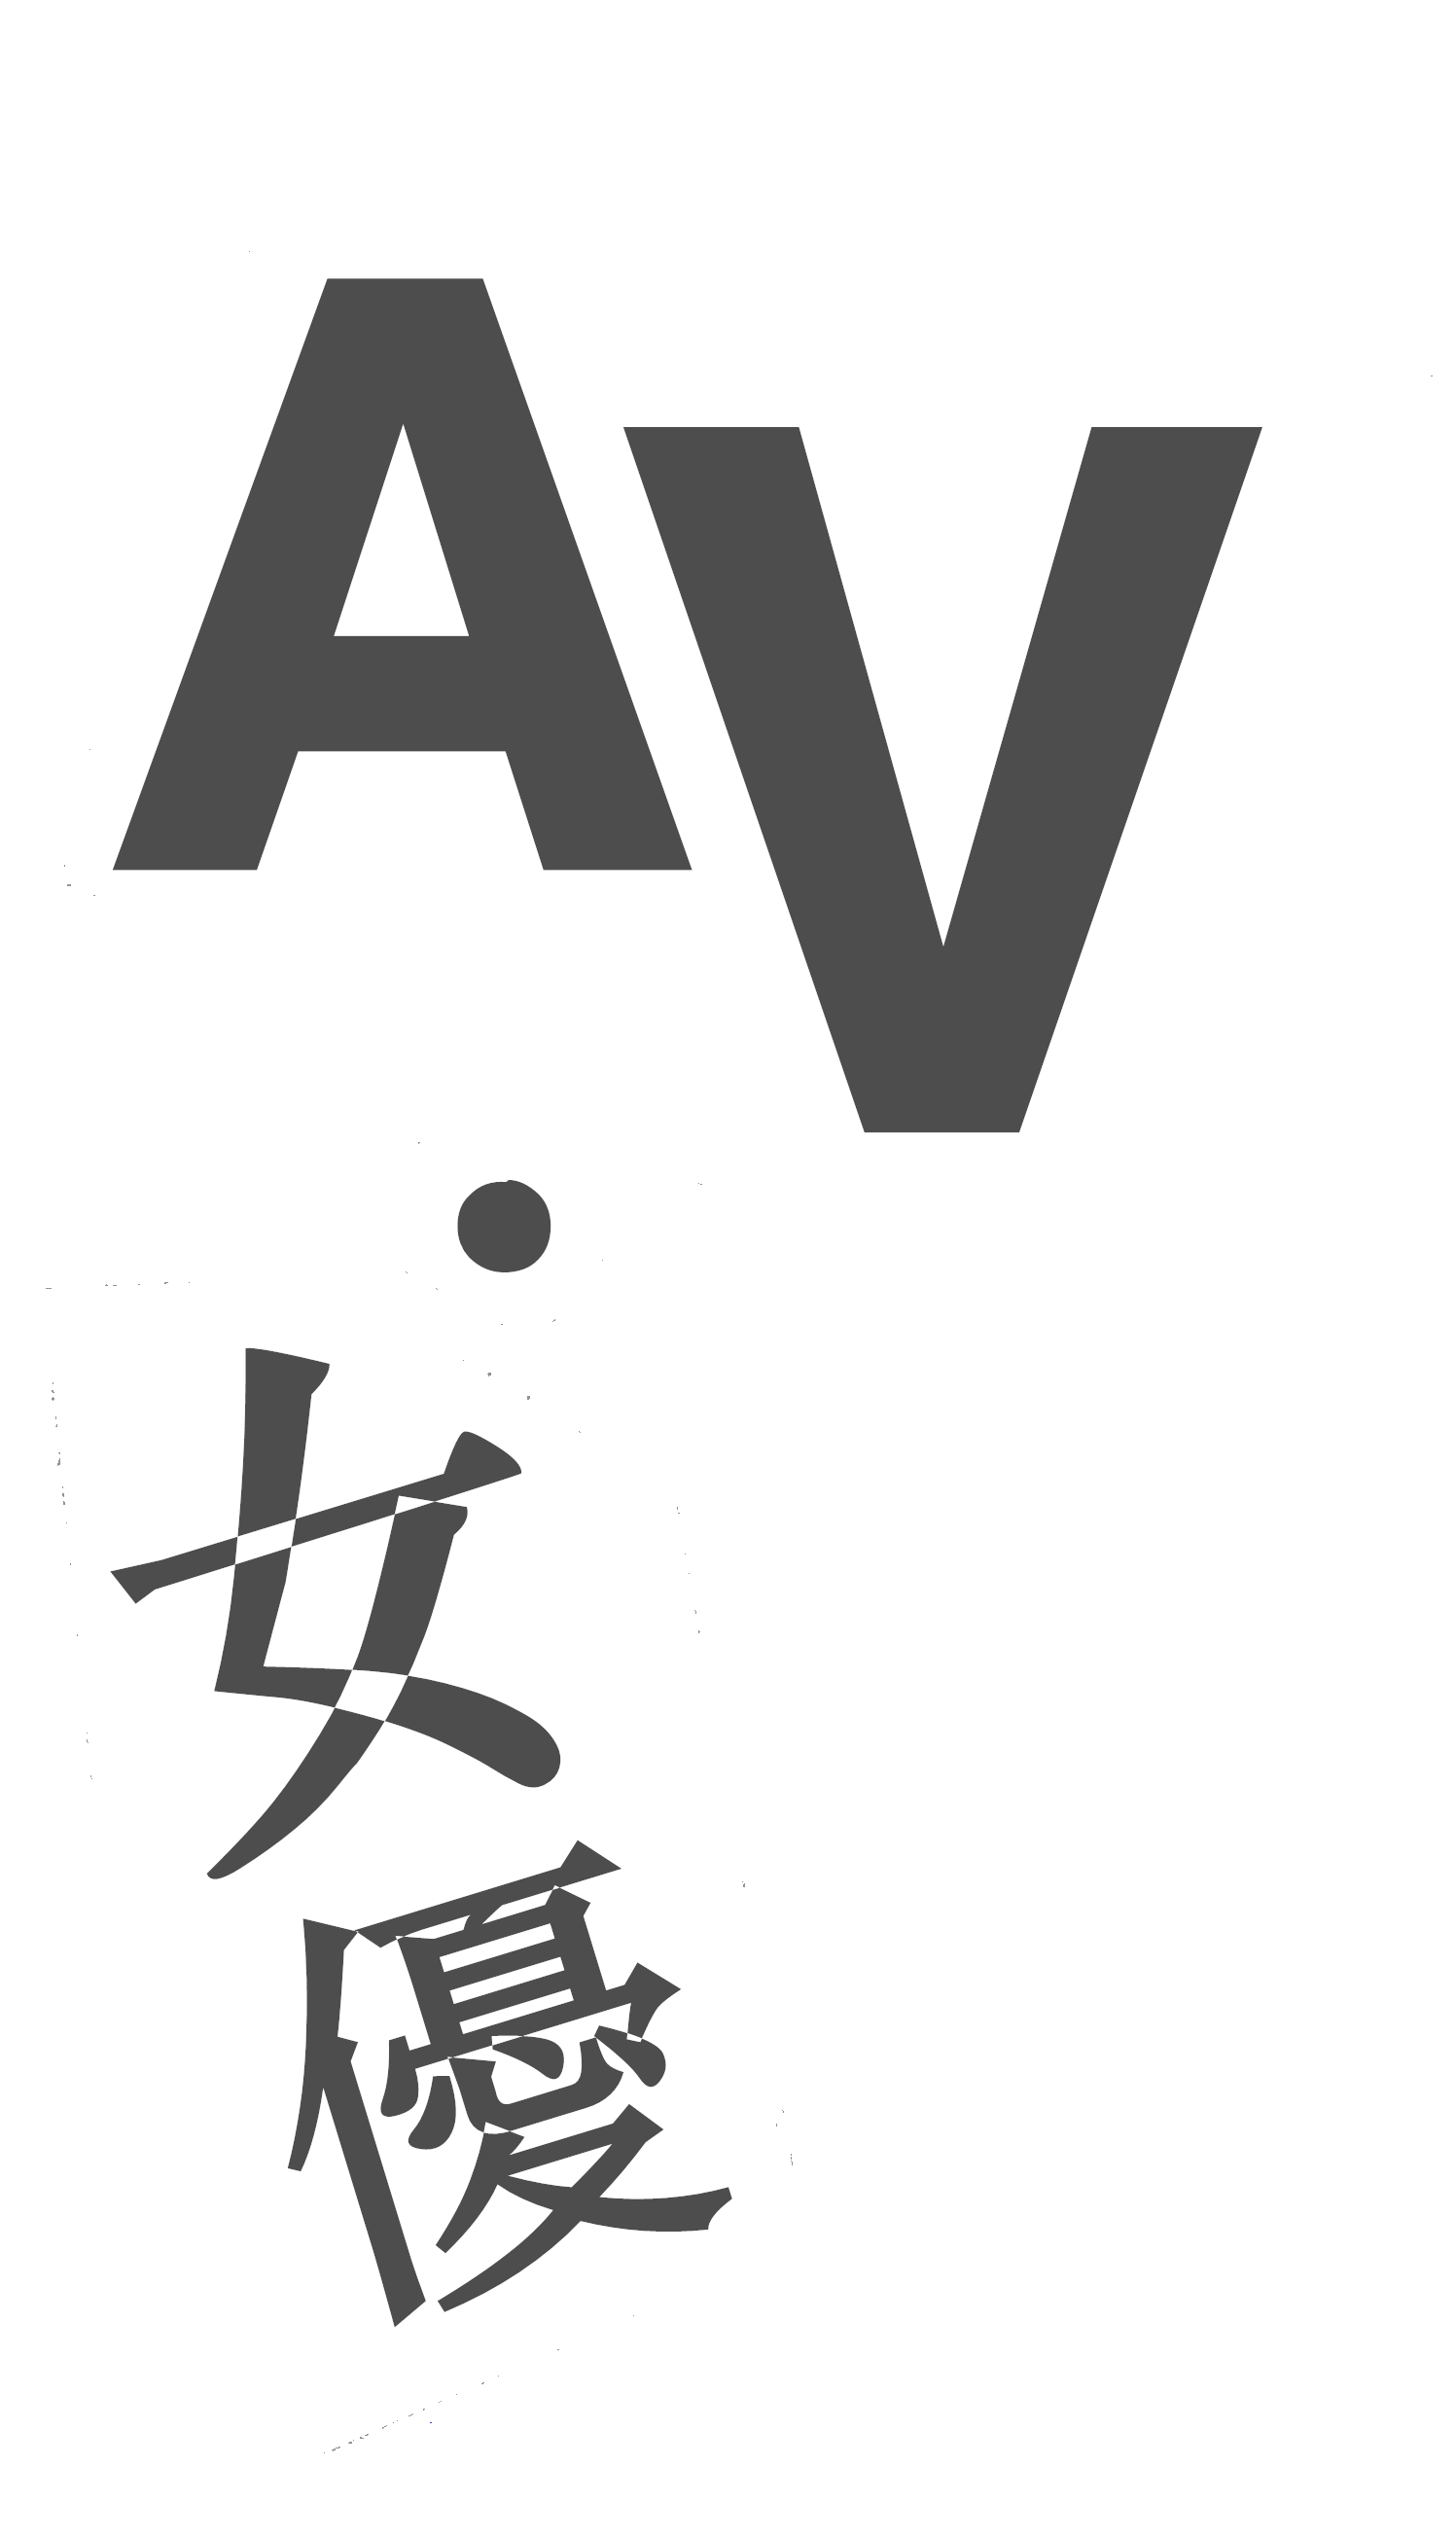
\includegraphics[width=0.7\linewidth]{ch01.png}
	\caption{第1章 AV女优}
	\label{fig:ch01}
\end{figure}

\section{一年内淘汰八成女优}

我在日本A片界知名厂商SOD Create担任非执行董事，因此必须经常与片商的选角负责人开会。而选角负责人则是片商公司里对应经纪公司推荐旗下女优时的窗口。

经纪公司会大量提供自己旗下女优的「宣传照」资料，并且向选角负责人宣传该公司旗下女优，让她们为片商演出A片。

大多数状况下，「宣传照」都会附上女优的裸照，因此任谁只要看一眼就能知道女优的胸围尺寸和身材状态。

如果模特儿经纪公司认为「很看好某某女优」时，就会直接带这个女优访问片商，并当场接受负责人面试。换句话说，选角负责人对于业界内的女优动向相当了解。诸如SOD之类的知名大厂，更是收集了这个圈子里所有活动中女优的最新情报。

即便如此，选角负责人也无法在一年之内完全掌握刚出道AV女优的准确数量。若是询问：「现在究竟有多少位AV女优？」他们也只能摇摇头，因为这个数据相当庞大，常会不断攀升。

在这里我来稍微推算一下。

首先是经纪公司的人数。大公司的女优数量会超过100人，中等规模的公司最多会有50人左右，而小公司通常则不到10人。而全东京都内的相关经纪公司全部加起来，大概有100间。

在这100间公司里有五间大公司，因此女优人数就会是100人×5间公司，等于500人的数量；中等规模的公司为20间×50人等于1000人；小公司则是70间×10人等于700人。因此将全部数据加总，便有2200位AV女优。

虽然这只是估算出来的结果，不过我是以合乎业界现况的观点来计算，所以这个数据不会有太大的误差。

从估算的结果可以知道，目前总共有约2000名女性以女优的身份在这个业界里「活动」。根据A片作家藤木TDC先生的《成人影片革命史》记载，从2009年到2013年，平均一年有1万部以上的A片新作上市。虽然书里没有确实刊出每年的新作数量，但我个人也认为这个数据相当合乎实际情况。换言之，A片界会动员2000名女优拍片，并形成一个每年可以制作、贩售一万部以上A片作品的大市场。

只是，可别真的认为这个圈子平时就一定有2000名女优在台面上维持运作。虽然有一些人气AV女优可以保持一年100多部主角级作品的拍片量，但其他大部分女优不但默默无名，只能拍些小规模的街头搭讪，其中甚至有人完全接不到工作。

此外，最重要的就是在2000名AV女优里，大约有八成会因为各自的理由，无法维持一年以上的工作寿命，就此退出A片界。不过，翌年女优人数依然会补充到原来的数量。

\section{AV女优多半经济拮据？}

AV女优分为三种，分别是「单体女优」、「企划单体女优」、「企划女优」。

「单体女优」是一种会被片商提拔成主角，能将个人的照片印在商品包装上，而且也有能力让固定客层形成粉丝团的AV女优。由于这类女优大多都是在业界中被认可为等级较高的族群，所以会与特定片商签下专属契约。而「企划女优」若是要用直接一点的说法来解释，就是商品价值上与单体女优相比，较难自成气候，通常都是接演《女子性爱温泉旅行大会》等有多位女优同时登场的作品，有时她们的艺名甚至不会印在商品包装上。在2000名现役AV女优中，大约有九成都是「企划女优」。

「企划单体」就是有着「单体女优」的超高人气，却没有和片商签下专属契约的女优。由于她们不受契约约束，所以能自由接演各片商的A片，因此作品数量往往可以迅速飙升。

目前会将AV女优的工作当成主要收入来源的人，大多都是「单体女优」和一部分「企划单体女优」。由于每位AV女优在刚出道时，都无法确定自己能否大红大紫，因此几乎全部的女优都会从事其他工作。对她们来说，那些工作反而比较像是「正职」，而AV女优顶多只是一种赚外快的「兼差」。

万一没办法在1个月内推出3部以自己为主角的A片，那么单靠当AV女优来过生活的计划将会走得极为艰辛。所以一旦卖座女优的人气过了高峰期，就该考虑放下自己的身段，试着改变戏路以配角的身份继续维持自己的职业寿命。

由于女优间有激烈的生存竞争，因此大概有八成左右的女优会在竞争中遭到淘汰。她们通常不到一年时间就会退出A片界，回到一般社会里继续过生活。

\section{锱铢必较的成本管控}

我经营的制作公司目前每个月可以拍出十部A片，而每一部新作正式贩卖时，都会在光碟正面印上「溜池五郎」的名号。

当我的制作公司从物流、贩售的客户手中取得制作费时，就会将这笔资金用于摄影、剪接，甚至是商品包装的设计上。当然，所有拍片经费包含我的导演酬劳也必须在这个预算范围内。

不将AV女优的片酬计算进去的话，目前拍一部A片的总预算，不分作品种类大概都是在100万至150万日圆以内。

这笔费用会用在摄影师和专业造型师的酬劳、商品包装设计上，当然也会用在摄影棚的使用费、拍片当天的各种杂费、女优的治装费，还有AV男优的片酬上。

至于AV女优的片酬严格说起来不是由我们直接支付，而是将片酬支付给她们所属的经纪公司。有时女优一整天的片酬约莫20万至30万日圆，有时价格甚至更高。

\section{拍片中没时间吃晚餐}

前文中有提到以目前的行情，若没办法在一天内拍完一部片，就会超出预算。

其中最耗预算的就是摄影棚的使用费。由于我常常拍摄人妻类作品，因此必须使用备有厨房、客厅、和室、卧室的住家型摄影棚，另外也有租金1个小时以数万日圆计算的摄影棚。

在我的工作现场中，大家会固定在早上集合。而女优也必须当场让造型师做好造型，直到下午一点前都是拍封面照等相关的摄影时间。简单吃完午餐后，就会正式开拍，剧本里的全部场景必须在9小时之内完成。

晚餐时，导演助理会将便当放在餐桌上，大家会找时间自行用餐。事实上，拍片时从来不会轻松悠闲地吃饭，也完全不可能出现慢条斯理、谈笑风生的景象。

工作人员中尤以AV女优最为辛苦。因为她们诠释性爱的演技堪称「重体力」，除了要在数小时内频繁演出性爱场面外，每次性爱场面都得持续一小时以上。

至于低预算的拍片现场大多不需要这么辛苦。一部片的预算通常不超过50万日圆。

\section{女优看实力，片商看数字}

AV女优从以前就不是光靠可爱美丽的外表来维持人气，想从事这一行就该彻底奉行实力主义。而女优想要在自己的作品中展现实力，获得粉丝们的青睐，就得靠不断自我推销。

虽然「单体女优」会和特定片商签下专属契约，但这个时期就算出道作能大为卖座，到了发第二部作品时销售数字还是会明显锐减。眼见这样严苛的情势，有许多女优们通常也会有自知之明，努力拍片。

但片商却大多只看女优的销售数字。换句话说，他们通常只看销售量来评价一个女优的好坏。

\chapter{第2章 私生活}

\begin{figure}[htbp]
	\centering
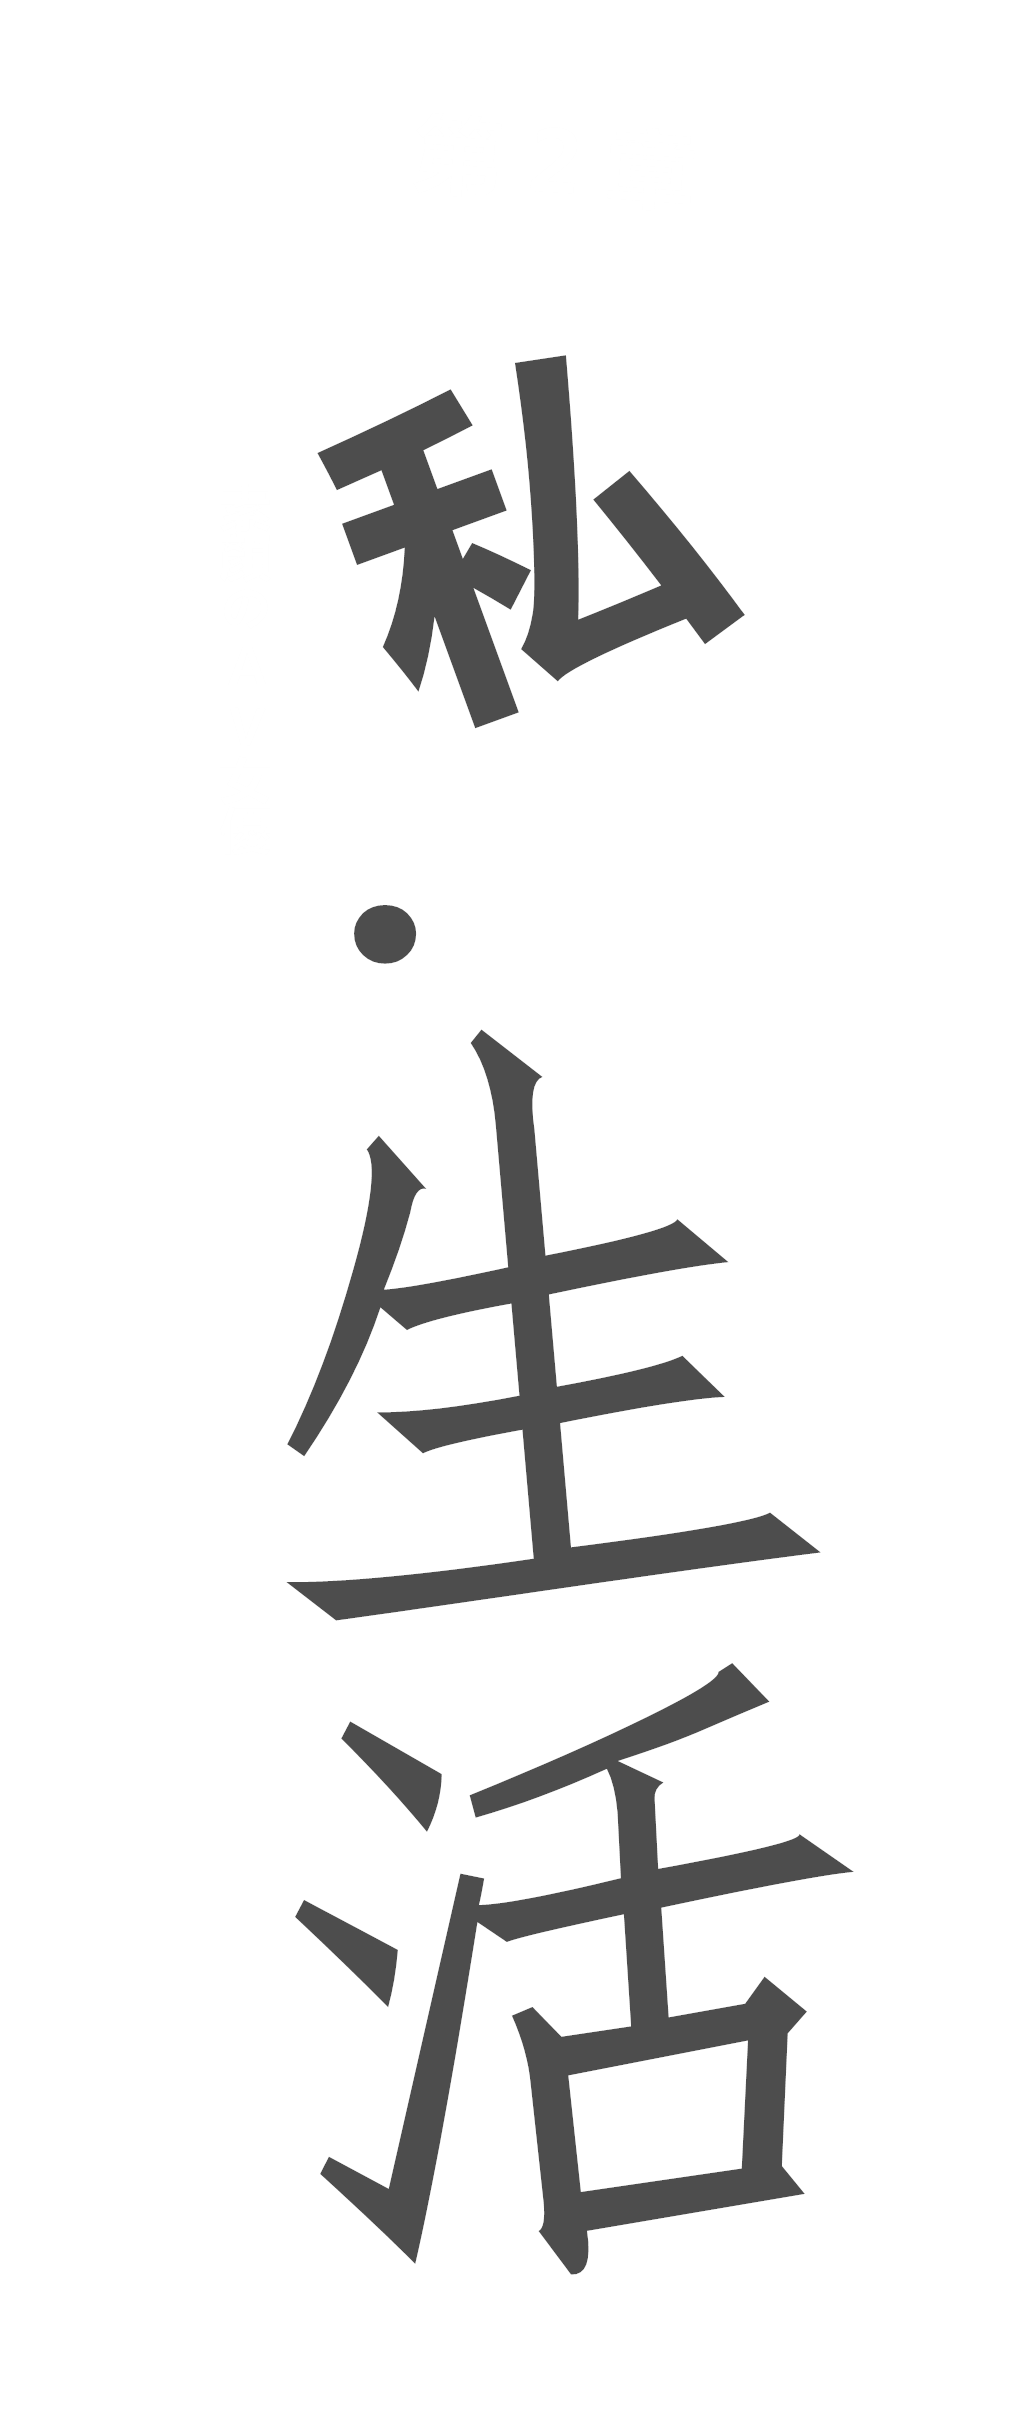
\includegraphics[width=0.7\linewidth]{ch02.png}
	\caption{第2章 私生活}
	\label{fig:ch02}
\end{figure}

\section{AV女优也是普通女性}

1996年，「援助交际」入选日本流行语大奖，再前一年登场的则是「男来电，女来店」。就在「援助交际」突然在日本全国各地普及开来，也被用来代称女高中生以肉体换取金钱的「卖春」行为时，渐渐也开始有一部分粉领族和成熟妇人习惯用「Support」作为卖春的行话。

虽然在这个时期我早就已经是一个A片导演，但就在我也注意到援交风气蔓延开来的20世纪90年代后半，应征AV女优的女性确实有显著增加的现象。

当然我也认为那些前来应征的女性不见得全都是有过援交经验的人，但当女性知道能藉由做爱轻松赚取金钱，前仆后继争相触犯出卖灵肉的禁忌后，自然也就会认为演A片也是其中的选项之一。

只是，若是自己演过A片的事被自己的父亲、同班同学、男朋友发现就糟了——她们多半都是用这类理由来打退堂鼓。

反观A片的拍片现场，不但会有签约经纪公司派出的经纪人陪同录影，导演、摄影师等全体工作人员也只会用淡然的态度进行拍片工作。至于男优大多都是很习惯对待女性的老手，态度上其实都相当绅士。男优们平时也都会定期做好性病相关健康检查，所以援交在安全性上根本没得比。

如果问我：「AV女优和一般女性有何差别？」，那么我会毫不犹豫地回答：「就差在愿意抛头露脸的决心。」

\section{AV女优也是种职业选项}

即使女优在片中现身演出，我们也是有办法让她们的确切身份不至于曝光。A片业界会如此小心谨慎，就是为了保护女优个人的身家资料。

在我们这个圈子里，会将演A片被亲朋好友发现的状况称为「父母抓包」、「男友抓包」。

正因为A片界对女优有着如此无微不至的保护，所以女优们可以不在乎自己一丝不挂的模样被他人指指点点，进而让这个业界每年都有将近2000位女优出道。

\section{各种拍摄A片的动机}

我的部落格和脸书偶尔会有粉丝留讯息问我：「AV女优到底有多好色？」

虽说拍A片只是一种工作，但AV女优中的确有许多人具备好色的性格，在性爱方面也颇有历练。就算只是单纯「想靠这一行赚钱」才决定进入A片界，但若是本身对性爱没兴趣，也没有高明的性爱技巧，那么出道后肯定无法持续下去。

其实有些过着无性生活的太太、拥有异常性癖的粉领族对AV男优的演技相当感兴趣，她们正是那种「希望能安全享受性爱」的族群。我个人认为无论是「金钱」还是「性爱」都是不可或缺的入门因素。

\section{女优的正职工作是？}

在前面我提到过大多数女优都有自己份内该做的「正职」，平时都是利用周末和假日拍摄A片。

虽然她们来自各行各业，但大多女优的正职都是护士。我无法分析为何护士会占多数，不过我想这应该和她们平时有严重的工作压力有关吧。

女优以自己的正职为A片卖点时会有一种特征，那就是话题性来得快，去得也快。而她们也了解自己一旦被身边的人「抓包」就该马上从A片界引退。

其他还有补习班教师、空服员、百货公司的专柜小姐、企业经营者等等。总之这个圈子的部分女优本来就有收入稳定的职业。

\section{短期离乡的拍片生活}

有些AV女优习惯平时在自己老家安静地生活，需要拍片时每个月就抽出一个礼拜的时间到东京，并且在这七天的时间内密集赶完拍片行程。这一类女优在最近的五年有明显增加的倾向。

会形成这样的风气，其实是因为东京都在2008年时修改了《迷惑行为防止条例》。随着这项法律的修改，从新宿到涩谷的路上，禁止任何人向一般女性搭讪，也不准A片业者在路上找寻明日之星。

所以，取而代之的就是经纪公司在网路上发布求才广告。

\section{引退和复出间的挣扎}

「传说中的女优重出江湖」。看到商品包装上这句斗大的标题，就知道是当年颇具人气的女优再次复出。

\chapter{第3章 美熟女}

\begin{figure}[htbp]
	\centering
	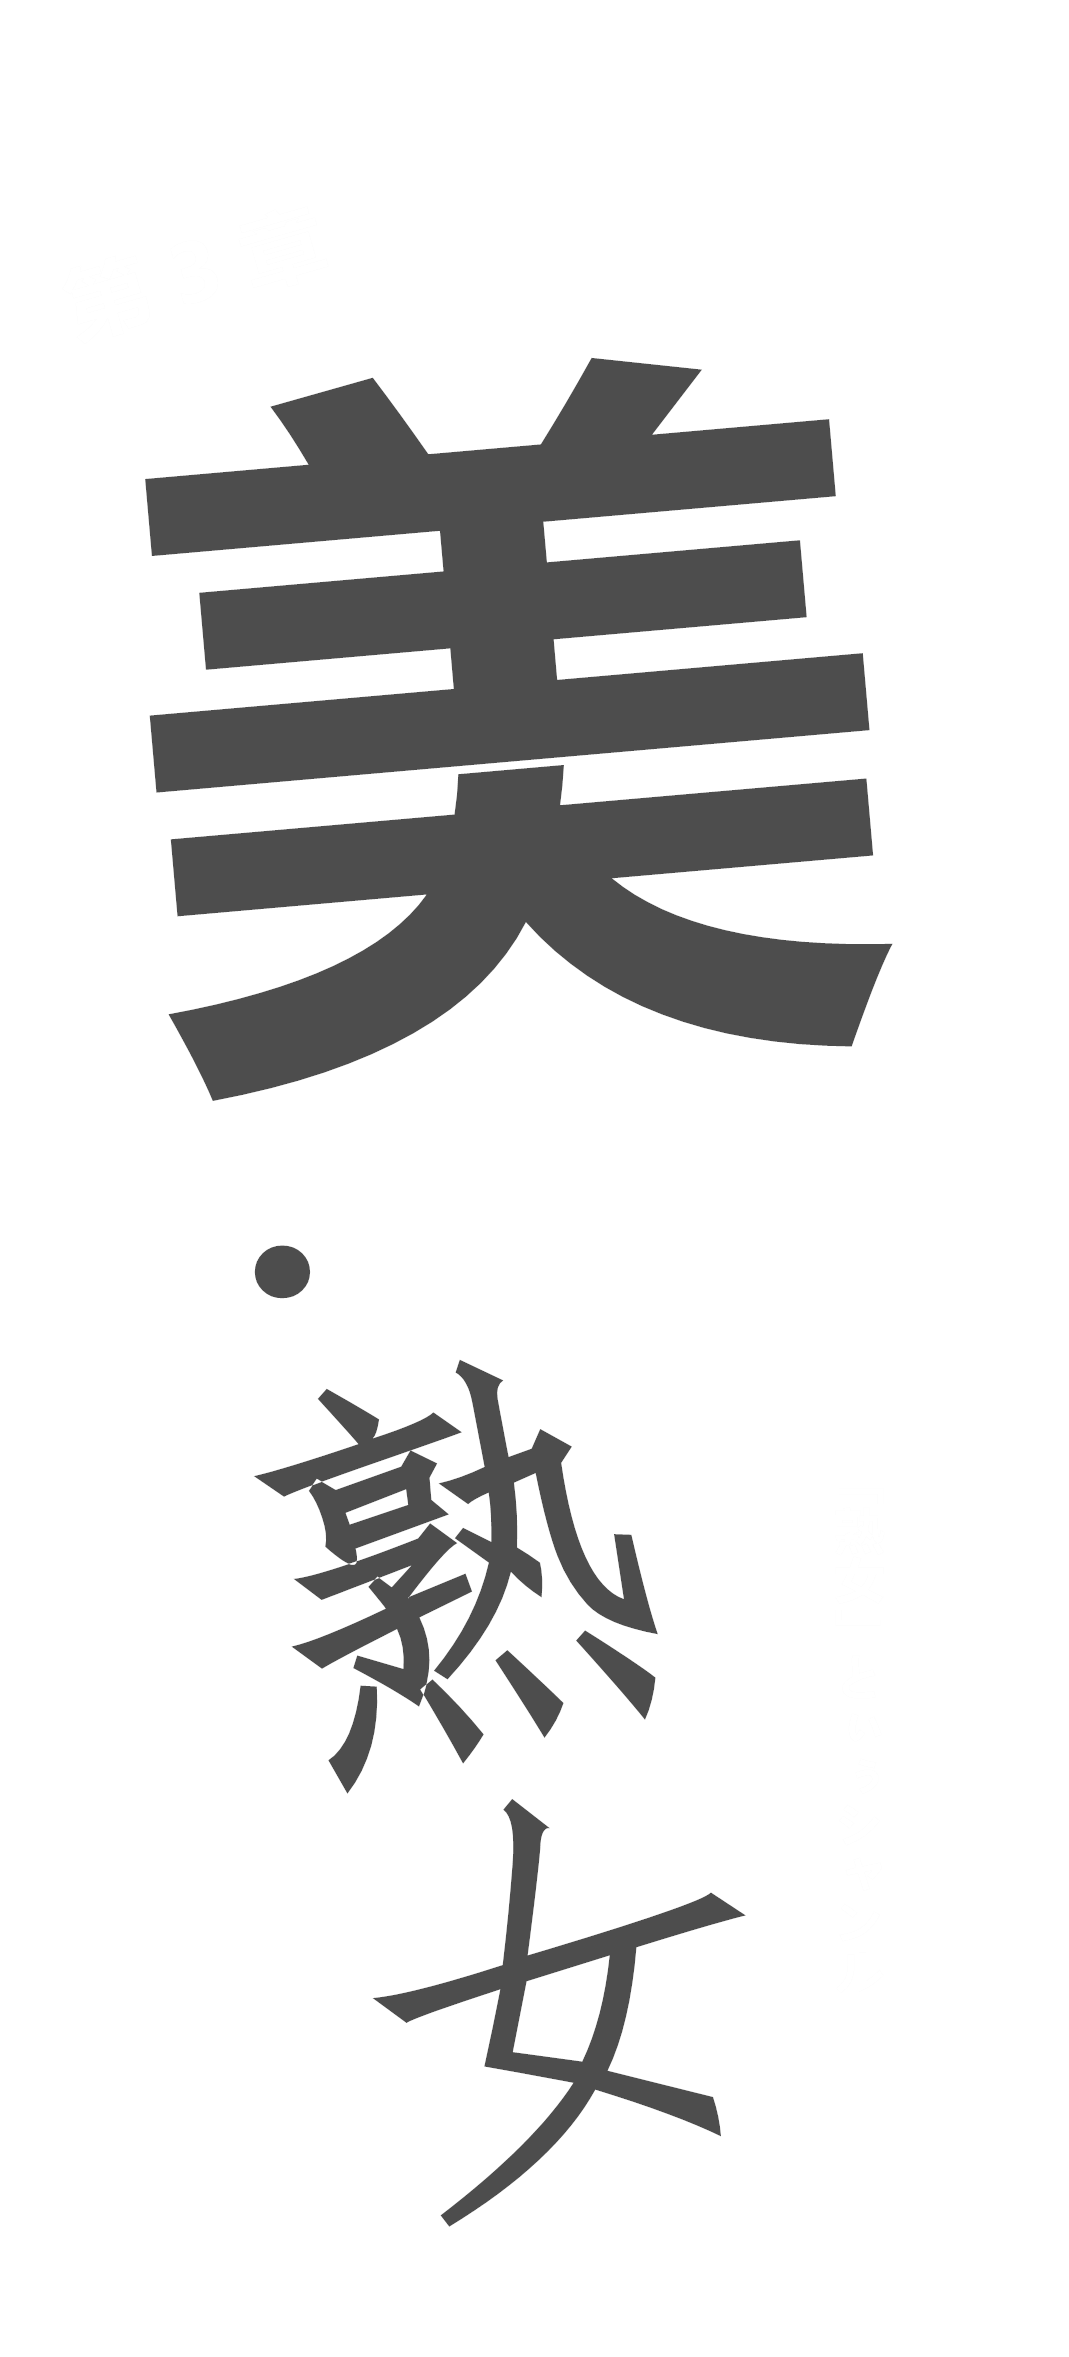
\includegraphics[width=0.7\linewidth]{ch03.png}
	\caption{第3章 美熟女}
	\label{fig:ch03}
\end{figure}

\section{不想老是当某人的太太或妈妈}

12年前，也就是2001年时我曾拍过《人妻羞耻部屋》系列作品。这个系列在选角时，都是以身材有点走样的女性为主角。女优的特征就是虽然有着巨乳，但肌肤仍保有20岁时的弹性，毫无姿色，满肚子赘肉。不过A片主题却隐含着「美熟女」从年轻开始就有办法随意摆布、玩弄男性的性暗示。

我曾经为了追求真实感和临场感，故意在女优不知情的情况下让门铃突然响起，使女优以近乎全裸的姿态面对突如其来的状况。

这位女优——木下由香里（化名/当时31岁）却因为这突如其来的发展而哭了起来。

木下是一个育有孩子的妇女。但是自从当母亲以来，附近认识的人、自己的朋友都不再叫她的名字。无论何时何地，都称她「〇〇太太」和「〇〇妈妈」。任何人都这样叫她，当然，身边的亲戚们也会如此称呼木下。但是这对女性来说，就等于是否定身为女性的身份。

自从生过小孩后，妊娠纹早已经藏都藏不住。不但胸部下垂，还因为喂母乳的关系让乳头变黑变形。

我对着满脸泪水并且充满困惑的木下说：「我可以从你变黑的乳头和妊娠纹感受到你的性感，所以我才会决定一定要由你拍这部片子。」

\section{27岁以上的女性就是「欧巴桑」}

过去A片界会把超过27岁以上的女优称为「熟女」。2000年前后，我为SOD导演的所有作品都是以熟女为主角。由于这样的选角在当时是一种违背常理的异例，因此偶尔会有业界人士嘲讽：「溜池五郎脑子不正常了。」

打从娘胎出生以来，我就是一个对熟女魅力有无限遐想的男人。要是无法拍出一部忠于自己性癖的作品，就代表自己没资格当一个A片导演。

就在那个时期，SOD的高桥雅也先生对我说：「拍你想拍的片子吧。」事实上，我是在SOD主办的麻将比赛认识高桥先生。由于他能理解我想拍的A片，因此才会诞生由川奈真里子主演的《义母～真里子34岁～》。

这部作品不但在1999年发售当时造成热卖，同时也确立了「美熟女」这个新属性。

\section{经济发展与人妻性爱的关系}

当熟女风潮开始在A片界萌芽时，社会上又有什么样的变迁呢？

这段期间被称为「失落的10年」（1991年3月至2002年1月），是日本经济低迷期的末期，当时社会气氛显得有些悲观。

在社会经济状态良好时，女性不用特别努力也会有男人来讨好自己，所以在性爱的过程中难免会出现「偷懒」的行为。相对地，在经济不景气时，女性就不得不拼命一点，让自己不会被男人嫌弃。

所以，男人负责送钱、送车、送化妆品的时代已经过去，紧接着的是女性若不在性爱上满足男性，想要的东西就无法到手的时代。

\section{肉食系熟女天后}

到了2008年，有一位性爱技巧凌驾于所有女优之上的肉食女米仓真耶突然在业界中崭露头角。

米仓是我个人专属A片品牌「溜池五郎」的第二位女优。从远方看起来，就像是有着黛比夫人的威严和妖艳气息的20多岁女性，至于身材则有点丰腴。

其实米仓在我的品牌中出道前，曾在某间知名片商的面试中遭到淘汰。不过当我拿到宣传照的那一瞬间就觉得惊为天人，然后要求经纪人安排演出的合作事宜。

米仓在面试时经常会「啊哈哈哈哈哈」地咧嘴大笑，这种笑声听起来实在是既爽朗又快乐。也因为这样的笑容，我当场决定请她和我们合作拍片。

就连拍片时都能展现出异于常人的肉食系性爱，我认为她可以说是一个最适合诠释榨乾男优演技的女优。「熟女+肉食系」，若说这个全新的女优属性和A片市场是在此时俨然形成也不为过。

\section{和儿子的朋友发生性关系}

关于本篇要讲的故事，虽然是我在拍片现场以及「导演面试」中，从女优口中听来的，但基本上女优本身的私生活细节我通常都不甚了解。

2008年，石本佐江（化名/当时46岁）由某个片商负责人带来面试。

虽然还未撤掉丈夫的户籍，但双方早已长年分居。而夫妻不合的原因就是和丈夫、儿子的贫困生活让石本觉得很有压力。

但是，石本仍然忘不了外遇后发生性关系的愉快经验。所以44岁时又和一个年轻男人婚外情。但是这次的对象却是儿子的同班同学，而当时他还只是一个18岁高中刚毕业的年轻人。

\section{报复丈夫外遇的人妻}

如果能在「导演面试」时让人妻型女优卸下心防，面谈内容就会有180度大转变，她们多半会开始发泄关于丈夫的牢骚。

牢骚之一，就是夫妻之间无性生活。丈夫不但不把自己当女人看待，也有好几年的时间没有过肌肤之亲。

在性方面和丈夫产生障碍的人妻型女优里，有位真田有美（化名/当时35岁）女士。她有着鸭子嘴和纤瘦身材，但指甲上华丽的彩绘让人看不出是家庭主妇。

她就是因为丈夫外遇，才会在愤怒之下要求演出A片。

\chapter{第4章 秘业界}

\begin{figure}[htbp]
	\centering
	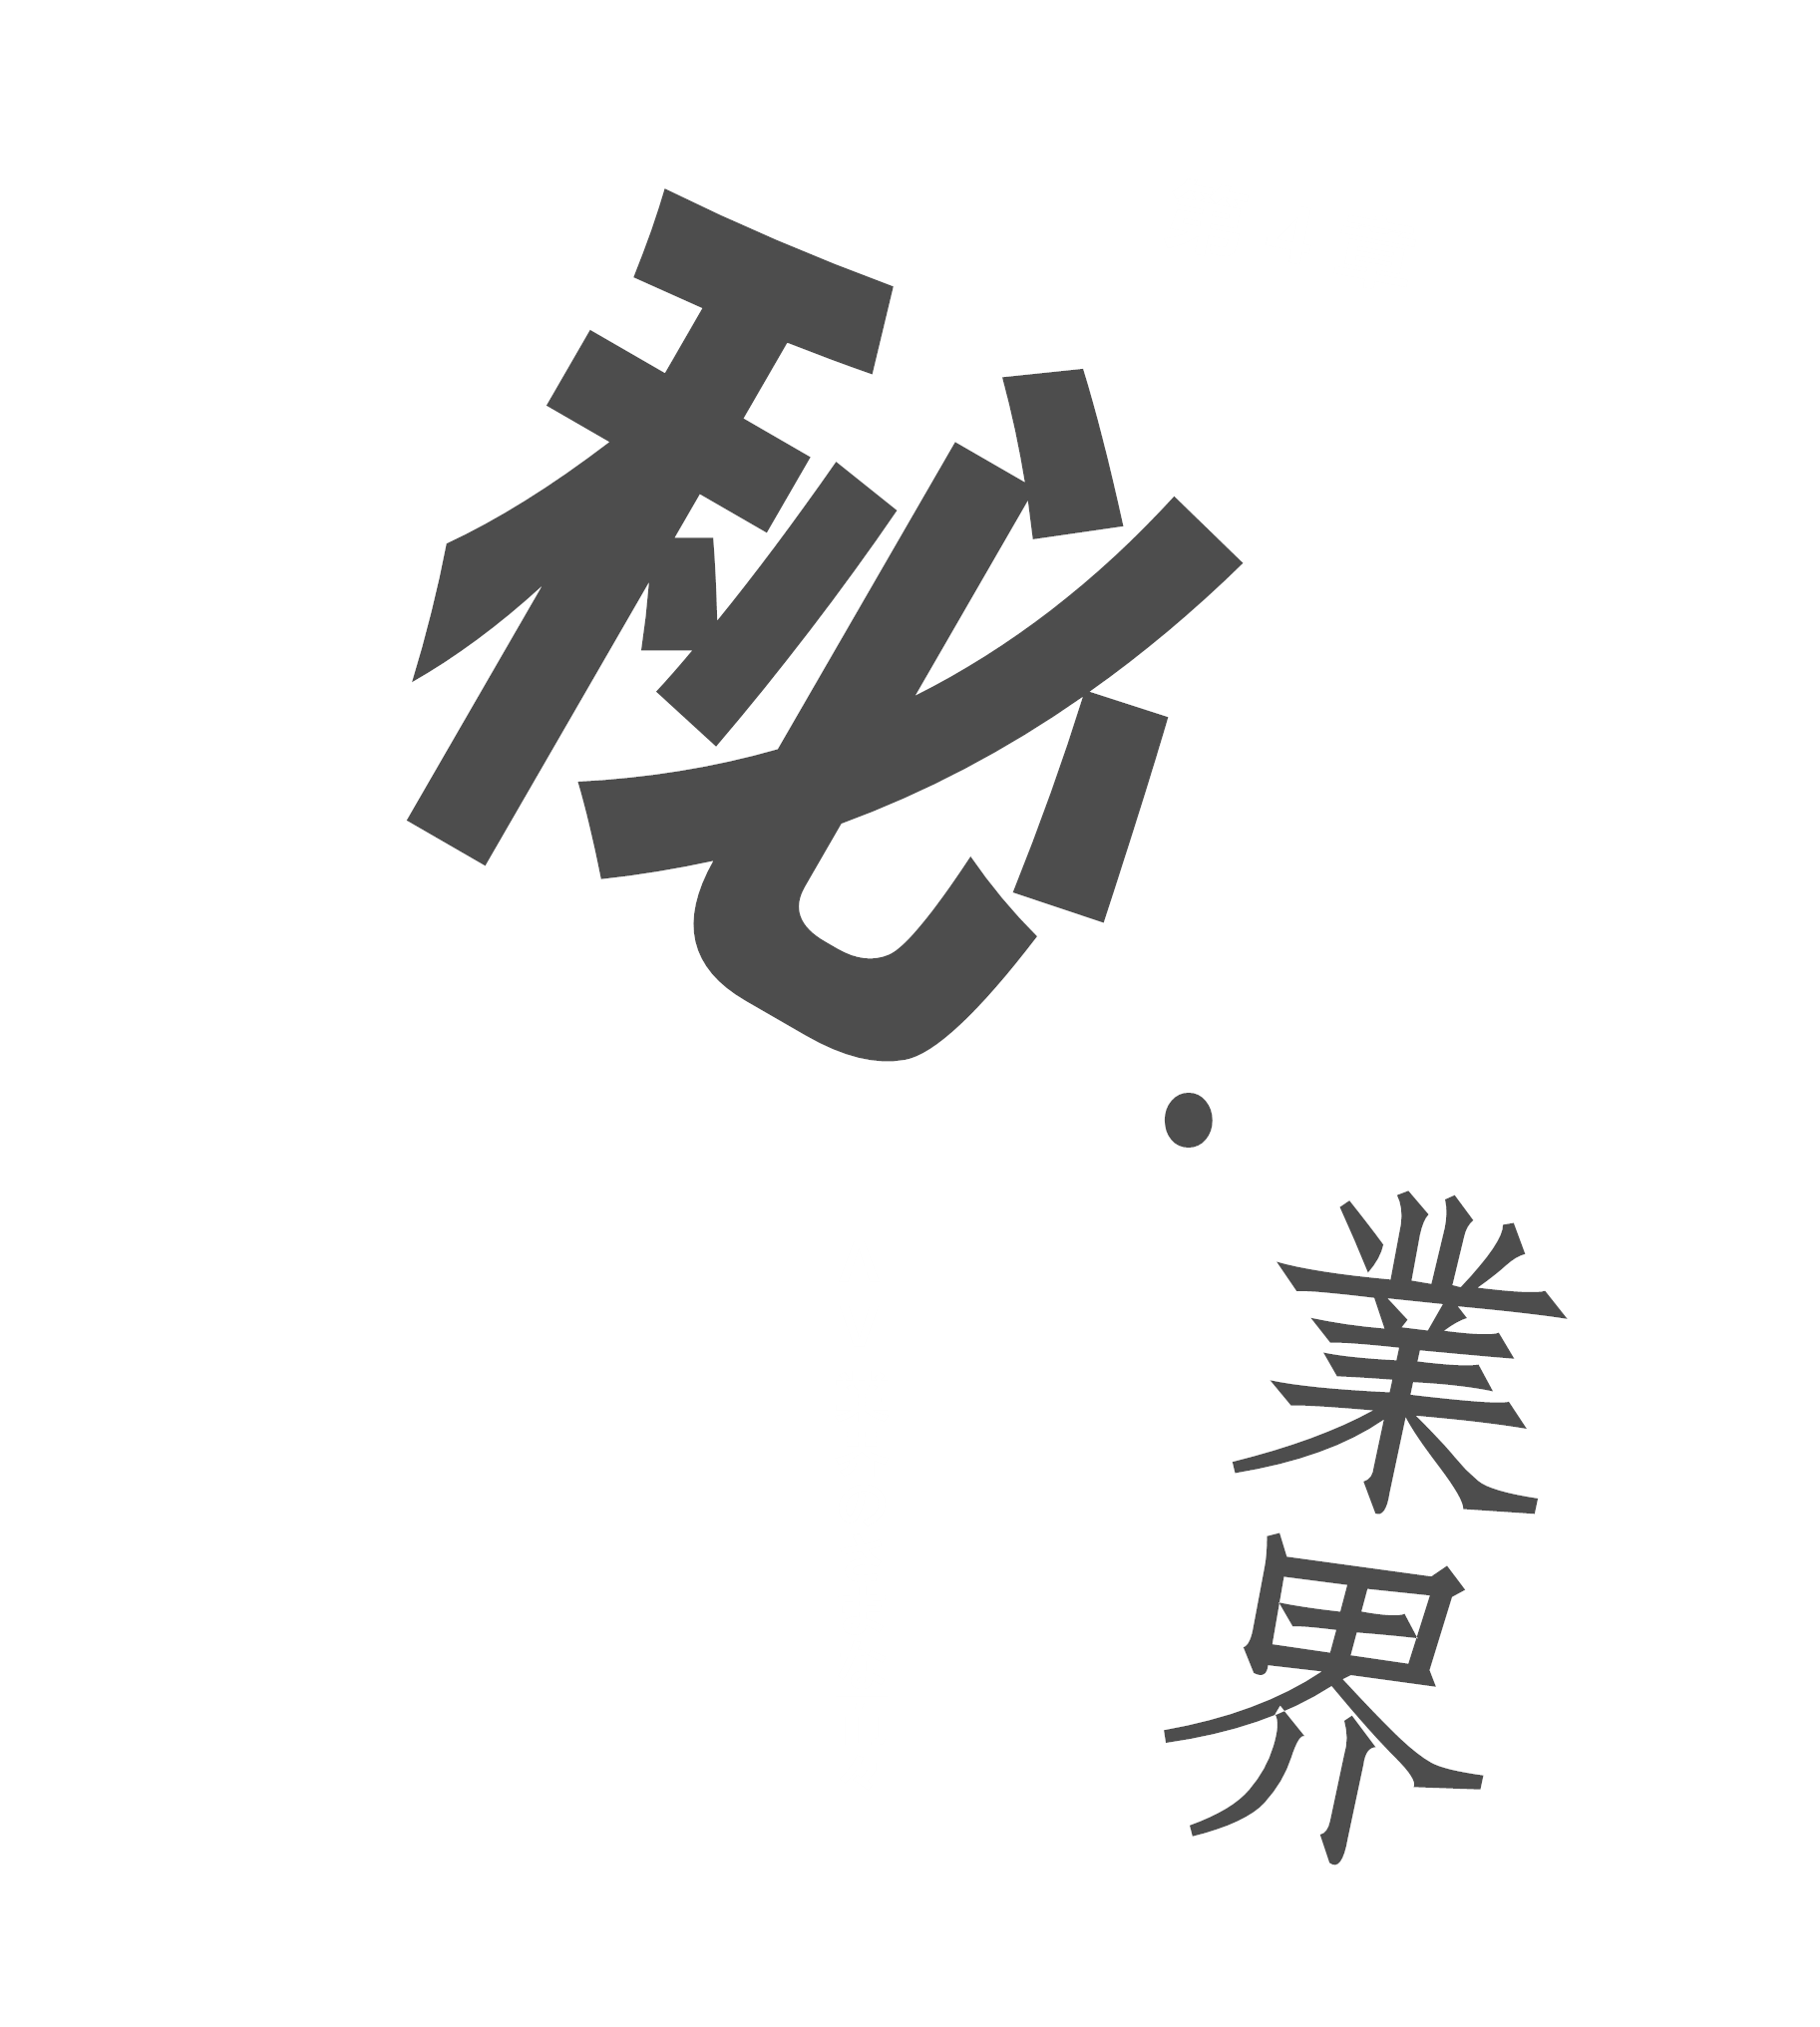
\includegraphics[width=0.7\linewidth]{ch04.png}
	\caption{第4章 秘业界}
	\label{fig:ch04}
\end{figure}

\section{神秘的发售方式}

AV作品的销售方式一直在变化。从最初的录像带出租，到后来的DVD直营，再到网络下载时代。A片业界随着科技发展不断调整销售策略。

片商除了一方面要拼命说服店家「本社作品保证卖座」外，另一方面还要不断拜讬卖场，确保自家商品每个月都能在卖场的货架上占有一席之地。

\section{业界的人脉关系}

AV业界是一个讲究人脉关系的封闭圈子。从导演、摄影师到女优、经纪公司，每一个环节都紧密相连。

经纪公司会大量提供自己旗下女优的「宣传照」资料，并且向选角负责人宣传该公司旗下女优，让她们为片商演出A片。

选角负责人对于业界内的女优动向相当了解。诸如SOD之类的知名大厂，更是收集了这个圈子里所有活动中女优的最新情报。

\section{从企划到上架的流程}

一部A片从企划到上架需要经过多个环节。首先是企划阶段，导演和片商需要构思新的题材和卖点。然后是选角，挑选合适的女优来担任主角。

接下来是拍摄阶段，通常需要一天时间完成所有场景的拍摄。拍摄完成后是后期制作，包括剪辑、配音和特效处理。最后是包装设计和发行销售。

\section{宣传与行销的手法}

A片的宣传手法多种多样。除了传统的海报和广告，现在更多地利用网络和社交媒体进行宣传。

有些片商会举办女优见面会、签名会等活动来提升人气。也有些会在成人展会上展示新作，吸引经销商和消费者的注意。

\chapter{第5章 超禁忌}

\begin{figure}[htbp]
	\centering
	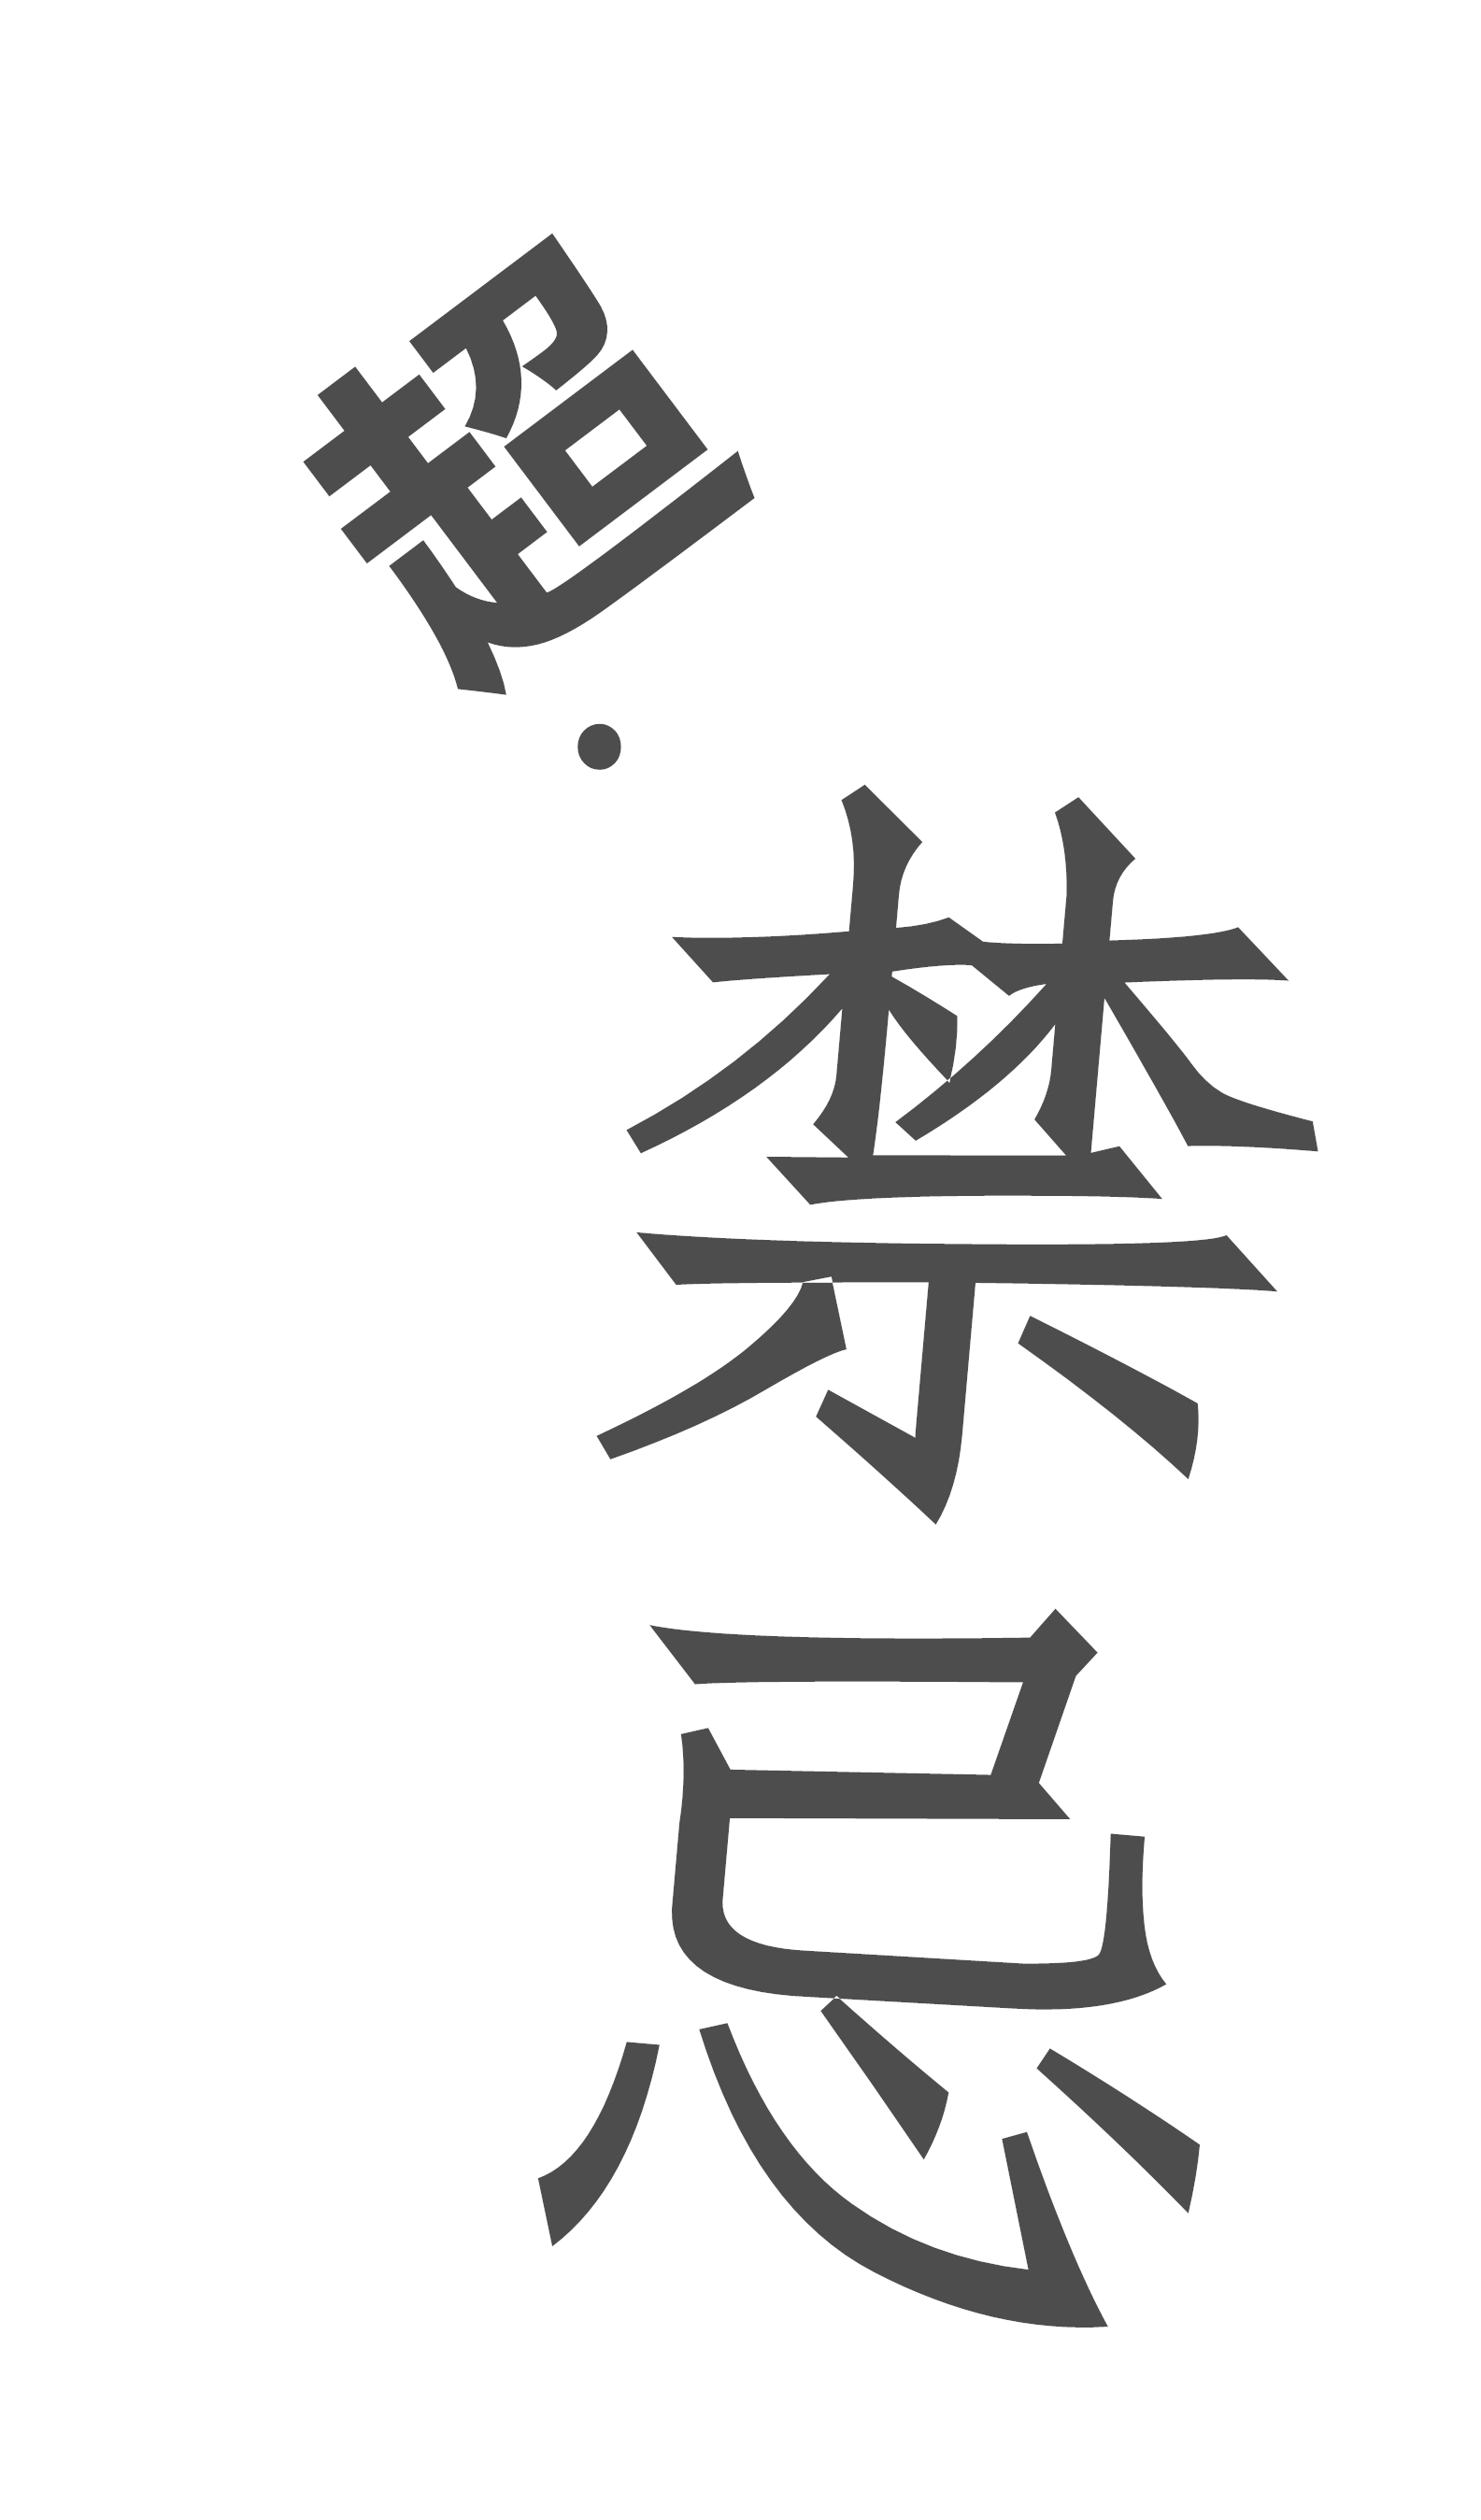
\includegraphics[width=0.7\linewidth]{ch05.png}
	\caption{第5章 超禁忌}
	\label{fig:ch05}
\end{figure}

\section{什么是「超禁忌」？}

在AV业界，「超禁忌」通常指的是那些挑战社会道德底线的内容。这类作品往往涉及伦理话题，引发社会争议。

但从另一个角度看来，这些作品之所以存在，是因为有市场需求。消费者的欲望推动了内容的创作。

\section{业界的道德底线}

虽然AV作品看似没有限制，但业界内部其实有一套不成文的规则。这些规则既保护女优，也维护行业形象。

「父母抓包」、「男友抓包」等状况是所有AV女优最担心的事情。A片业界会如此小心谨慎，就是为了保护女优个人的身家资料。

\section{禁忌题材的演变}

随着社会观念的变化，AV业界的禁忌题材也在不断演变。过去被视为禁忌的内容，现在可能已经成为常态。

例如，早期的A片很少涉及SM题材，但现在已经相当普遍。同时，一些新的禁忌题材也在不断出现，反映了社会对性观念的不断变化。

\section{女优的心理压力}

拍摄禁忌题材的女优往往面临更大的心理压力。她们需要克服自己的心理障碍，同时还要面对社会的眼光。

有些女优在拍摄完禁忌题材后会选择引退，因为她们无法承受外界的压力。这也是为什么禁忌题材的女优往往更加稀缺和珍贵。

\backmatter

\chapter{结语}

我和我的妻子，也就是前任AV女优川奈真里子育有一个独生子。

而川奈和我至今依然会在杂志等各媒体中露面，也会刊登个人照片于这些媒体中。我的妻子除了是前任AV女优外，目前同时也是散文作家、情色小说家，而我一直都是A片导演。虽说我的儿子还只是小学生，但多少也已经渐渐发现自己的父母所从事的职业。

我出版这本书的动机，就是为了这个目的。

这个身为A片导演的男人，与AV女优相识相恋，还成家立业。女人虽然从女优的身份中退休，但在孩子长大后随着丈夫以性爱和A片为主题，在媒体界打滚，并持续以此营生。

但从孩子的观点来看，我们的生活就和一般上班族、家庭主妇的普通生活没两样。工作之余，丈夫就只是一个宠小孩的「好爸爸」，会带小孩上柔道课、游泳课，休假时还会全家来一趟家庭旅游。

妻子骂小孩时会怒目圆睁，同时也会做家事、创作文章。——以上就是我和妻子平时的模样，是再普通也不过的生活。

虽然A片业界的工作就是拍摄男女做爱，并将这些影像商品化，但所有的工作成员，无论是片商的监制、制作人、宣传、演出的女优、男优、导演、摄影师、灯光、音效及造型师等，全都需要靠这种以「性爱」为商品的「成人影像」过生活。只是，一旦各自离开职场后，每人都有属于自己的家庭，只是一群非常普通的社会人士。

AV女优的「工作现场」绝对不是一群天天精虫冲脑、只想做爱的怪兽聚集的魔窟，只是一群再平凡也不过的社会人士专门从事性爱相关的「工作」场所。

不管这个社会如何看待，至少我和工作团队全体人员都十分乐在其中。

\chapter{延伸阅读：日本女优的结局}

我和我的妻子，也就是前任AV女优川奈真里子育有一个独生子。

而川奈和我至今依然会在杂志等各媒体中露面，也会刊登个人照片于这些媒体中。我的妻子除了是前任AV女优外，目前同时也是散文作家、情色小说家，而我一直都是A片导演。虽说我的儿子还只是小学生，但多少也已经渐渐发现自己的父母所从事的职业。

新时代的日本女优不再是缺钱、受虐的不幸女子的代名词，而是一批有着专业素养的职场女性。她们离开荧幕后，也会有自己的生活，有家人、丈夫、情人以及孩子相伴。但90\%的离婚率仍是摆在这些女优面前现实而残酷的噩梦。

溜池五郎不仅是一个人名，更是一个AV品牌——一个传统AV界的破局者。

在历经电视连续剧助导的工作后，溜池五郎于30岁正式以导演的身分进军AV界，靠着自己对AV的热爱，苦熬多年后终于获得观众的肯定与商业的青睐，成为了独立的知名AV片商。

溜池五郎这个日本AV界无人不知的名号，靠着他源源不断的创意，成功将一位又一位女优推至巅峰，更引领了日本AV界独树一格的拍片风潮。

20年间，溜池五郎投入AV拍摄的作品逾1000部，他用市场的反馈告诉了观众：AV的市场走向不再是以单单的肉戏才能博得眼球，与之相比更重要的则是剧情。

溜池五郎最为人熟知的作品便是熟女系列。有别于其它以童颜貌美女优为卖点的A片，在大多数AV导演对年轻貌美的女优暗自点头时，他把眼光放在了一个眼神就知道该干嘛的熟女身上。

1999年，他拍摄的《义母，真理子34岁》以熟女系列一炮走红，片中女主角川奈真理子也借此闯出了名号。

这位拍过千部AV的名导，略有涉猎的观众都会印象颇深，老牌、信用好，加之每一部AV的宣传封面上打着溜池五郎名号的人妻熟女系列，有底有料，且无论是视角观点，还是剧情走向，都在肉搏战中跌宕起伏。

作为AV导演，溜池五郎认为女优是一个值得尊重的职业，他也是少数关注女优们想法及生活的奇葩。

做女优，自然也是不容易的，除了要在镜头前酣畅淋漓的表演之外，颜值若是差了，一部片子拍出来，不会有什么波澜。

这其中，丰乳靠天生，美臀靠态度。这是溜池五郎在得知女优们在荧幕背后所付出的苦功后，在一次访谈中脱口而出的感慨。

溜池五郎认为，日本女优若是无法维持胸臀上的美观，那她就不具备当一个女优的资格。

事实上，每一个称职的女优为了维持自己有魅力的身段，都会夜以继日的苦心付出。每一个婀娜身姿的背后，都是一步一个脚印的汗水。

一旦成为当红女优后，辛苦程度更不是一般女优所能比拟的，说她们和演员艺人员相同等级也不为过。

日本每年的A片产量约有1万部，有2000名女优从事这一产业，这之间又有八成被凄惨淘汰。

自溜池五郎导演过的A片市面上已经超过了1000部，在这期间，他观察过许多女优，甚至有一位还成了他的妻子。

他有拍完片送花给女优致谢的习惯，最一开始，常有女优感动地流泪，渐渐的，他发现这些女优越来越习惯于带着微笑接过花束。

「这表明，她们现在已经认真的将拍A片当成工作看待，就跟一份正经工作没什么两样。」

专业的女优敬业且自爱。

\section{导演溜池五郎娶了女优川奈真理子}

1999年在溜池五郎的熟女系列《义母，真理子34岁》走红时，片中女主川奈真理子也一炮而红。

川奈真理子也是熟女，时年31岁，那也是她愤而投身女优行业的第一年。

令人津津乐道的是，数年后，川奈真理子与溜池五郎缔结了百年好合，两位在情海欲海漂泊的饮食男女凑到了一块，更是成了日本AV界知名的夫妻档。

在导演过川奈真理子的一次作品后，溜池五郎便向川奈真理子提出了约会请求，接着两人便迅速相恋。

这场毫不顾忌世俗眼光的恋情最终开了花结果，2004年，川奈真理子诞下一子。

\section{洗尽铅华改行当作家的女优}

结婚同年，川奈真理子洗尽铅华，选择隐退。

据日本媒体统计，自1999年跨入AV界，5年间她一共演出大约400部作品。

隐退之后，川奈真理子不想彻底放弃自己这5年的从业经历，学着自己丈夫开始了写书之路。

2011年出版长篇小说《继母的香艳》成功转型为作家，后来又发表了《禁忌——继母与婶婶与我》等多部作品。使她成为写限制级作品比较有名气的人物。

她的女性读者很多，这与同系列其他读物的受众群多为男性不同，展现在她女性读者面前的，是一个经验极其老道的熟女，自然她写的也更能戳进女性朋友的心坎里。

\section{如何向孩子讲述不光彩经历}

川奈真理子与溜池五郎的儿子今年也已14岁了。

在他10岁的时候，儿子某天问爸爸：「爸爸，你是做什么工作的？」

然而他很正经的回答了儿子这个问题：「爸爸的工作是AV导演，但你现在还不能看，要等到满18岁才可以看。」

儿子这时又问了：「是色色的东西吗？」

溜池五郎回答：「对，等你满14岁后，我会告诉你，同时还有你妈妈的事情。但是在那之前，你都不准搜索有关AV的事情，这是我们男人之间的约定。」

想来，他们的孩子现在应该知道自己母亲过往的职业了。

\chapter{读者感想}

\section{感想1}

本书，写的是AV女优工作现场实录。

我也是AV业界的从业人员，看完这本书后有一个感想，那就是：写出这些内容没问题吗？过去的AV和现今的AV的确有很大的差异，变化最多的就是「AV女优」。现在已经从过去「谁敢脱就能当AV女优」的时代，进化成没有任何企画的内容根本赚不了几个钱。

这本书是AV女优工作现场实录。

\section{感想2}

我自己也是女性，所以对于女性这样的生物，其实大概还能略知一二，所以乍听这本有关AV女优的书籍，其实并不觉得有多大的新鲜感。但我却特别对作者写到如果AV女优的「身体不好」就很难继续走下去这点，特别有深切同感。

读了这本书，觉得最厉害的是包含成人影带在内的所有演艺人员，这行没有强健的体魄是没办法做到的。

\section{感想3}

看完这本书后，对于AV女优们严苛的现实有清楚的了解。虽然我也只是单纯看A片的人，但也知道绝对不是长得漂亮就可以当AV女优。A片真的有一种不可思议的魅力！看完这本书，让我觉得自己看A片时可以更快乐了。

\chapter{名人推荐}

看日剧总会想知道导演是哪位，挑AV当然是先选对上眼的女优，不过，溜池五郎算少数的例外，这位拍过千部AV的名监督，牌子老、信用好。

溜池本人就是业界的传奇，这回由他来写AV女优的幕前幕后，不论是观点视角、近身接触，还是市场走势等等，专业权威，开眼界也长知识。

日本的AV女优约有2,000人，平均每年量产10,000部以上的A片，经济规模不小，竞争自是相对激烈，能存活下来，保有销售人气，无非就一个工作态度，把做爱视为工作，并不断揣摩演技。

拍AV的女优究竟怀抱哪种心境？只是拜金沉沦？宿命包袱？其实并不尽然，既成印象下的偏见或许扭转不易，但本书则能提供另一扇窗，让社会更加理解AV产业的存在价值，以及女优们在其职场上的敬业态度。

——小叶日本台

你以为在日本会去做AV女优的都是人尽可夫的浪女？你以为拍A片就是一男一女加一台摄影机就好？不要再傻了，人家能玩30年绝对没有那么简单，来看看「AV女优的工作现场」，你就能成为AV达人。

——一剑浣春秋

我们用右手实践幻想，女优用身体实现梦想，「快乐打炮、平安回家」，原来拍摄AV早已进化到再平凡不过的普通行业啊。

——亨利乳头市市长

成人产业是欲望为燃料驱动世界前进的火车，这本书就是撬开引擎盖让你窥看原理的实战手册。

——南宫博士

这些女优，拍了这么些作品，陪伴了我们整整好几世代的人，我总觉得我们欠她们点什么……

——雨狗 RainDog

\chapter{作者简介}

溜池五郎（溜池ゴロー/Tameike Gorō），1964年3月28日出生，毕业于明治大学法学院，日本AV导演。

\end{document}
